\resetfigpath{intro}
\glsresetall

\chapter{Introduction}
\label{intro}

The medical imaging field has recently witnessed the revolution of \gls{ai}, a broad discipline that is part of computer science, whose aim is to conceptualize human ``intellectual'' tasks, and produce computer programs that can replicate them, thereby allowing to relieve human beings from tedious and repetitive tasks.
From classification to segmentation tasks, \gls{ai} already provides flexible and efficient tools that greatly facilitate the daily practice of clinicians.
In particular, large quantities of \gls{mri} brain scans are now efficiently and accurately processed by \gls{ai} systems that help clinicians in the diagnosis of pathologies \cite{sun19}.
Similarly, surgical instruments can be segmented automatically and accurately in real-time to allow laparoscopic interventions of the abdominal cavity by means of robotic technology, thereby decreasing the invasiveness of traditional methods \cite{davinci}.

Before diving into the underlying intricacies of these systems, we
first wish to give the reader some insights on the genesis of \gls{ai}.
In particular, we describe the two main paradigms that are historically anterior to it, namely the descriptive and predictive analysis paradigms.
In a second section, we explain why one needs large amounts of annotated data to make \gls{ai} solutions practical, and how the medical imaging field, in particular, is hindered by this requirement.
Next, we emphasize how the present thesis aims at solving this issue.
Last, we give an overview of the organization of the present thesis.

\section{Descriptive VS. predictive analysis}
\Gls{ml}, a term that denote a sub-category of \gls{ai}, is grounded on the ``learning by example'' paradigm.
Whereas traditional approaches generally consisted in explicitly formalizing and implementing complex tasks as a combination of simpler programmatic instructions,
\gls{ml} rather considers that a flexible system can learn such instructions automatically through repeated experiences.
Formally, traditional computer vision techniques belong the descriptive analysis paradigm, whereas \gls{ml} relies on predictive analysis \cite{omahony19}.

The descriptive approach consists in producing a mathematical model that describes the considered phenomenon.
This requires to collect a representative dataset of the latter phenomenon, identify patterns (or features) that are relevant to the task at hand.
Next, a system is conceived that applies a set of rules to these features, in such a way as to produce the expected outcome.
The predictive analysis approach rather considers that the latter component can be obtained by means of a training procedure.
In particular, predictive analysis considers a model that includes parameterized mathematical operations. The training tasks consists in optimizing these parameters by minimizing an error, taken as a discrepancy measure between the system's output and the expected output.

To better illustrate the differences between the two approaches, let us examine a concrete scenario in which we are interested in elaboring a system that takes as input an image, and must provide at the output an answer to the question ``Does this image contain a car?''.
As a first step, we compute distinctive visual features, assumed to be relevant cues for the task at hand, e.g. large and homogeneous blobs (assumed to reflect the body of the car), and circular and dark-colored regions (assumed to reflect the wheels).
Both components are characterized by their size, orientation, and location.
A naive approach grounded on the descriptive analysis paradigm, would apply a serie of logical operations such as: (1) Are the wheels located below the body? (2) Are the wheels located at both ends of the body? (3) Is the average size of the wheels inferior to the size of the body? etc..
This toy example demonstrates how such an approach is often at risk of missing important and non-intuitive relations.
The predictive analysis approach aims at circumventing the latter risk by taking inspiration from the human functioning.
We humans can effectively derive the concept of car through experience, i.e. by being given a set of images that contain cars, and another set that do not.
The task of then resolves to inferring a combination of mental operations that would best separate the two sets of images.
This is often called the ``learning by example'' paradigm.

\section{On the importance of large quantities of annotated data}
\Gls{ml} methods, as the name implies, are built on the ``learning by example'' paradigm.
In their most primitive form, \gls{ml} methods considered feature extraction as a preliminary ad-hoc step, while the design and training of the model formed another step.
Engineers had to choose for the task at hand which features to choose, which was a tedious and cumbersome task.
More recently, thanks to the technical progress in computing hardware, \gls{dl}, which is a class of models that elaborate on \gls{ann}, brought the possibility to do end-to-end training.
In essence, \gls{dl} models allow one to optimize both the feature extraction module and the predictor in a joint manner, by regressing an objective criteria, also called loss function.
This has brought spectacular improvements in performance over traditional methods, making \gls{dl} the de-facto standard in most \gls{ml} fields.
As will be further developped in a next chapter, \gls{dl} models are composed of a concatenation of layers that each perform simple mathematical operations, such as matrix multiplication or convolutions.
The power, flexibility, and hence impressive performance boost of \gls{dl} models, namely comes from the fact that stacking layers allows to express complex and abstract features.

As showcase application, let us mention the ImageNet Large Scale Visual Recognition Challenge \cite{ILSVRC15}, which consists in classifying natural images into semantic categories such as ``balloon'', ``dog'', etc..
The training dataset contains $150'000$ images, classified into $1000$ categories.
As of today, the state-of-the-art performance uses a \gls{dl} model, in particular a Deep Convolutional Neural Network, which classifies unseen images with an accuracy of $88.6\%$ \cite{tan19}, a performance on par with human capacities.
The model, however, has over $70$ million parameters.
In this scenario, collecting such quantity of example images and annotating them is tedious and cumbersome.
In practice, the annotation task is performed by numerous individuals in parallel.

Another example scenario, more relevant to the present thesis, is the Brain Tumor Segmentation (BraTS) Challenge \cite{menze15}, which consists in segmenting brain tumors from \gls{mri} scans.
The training dataset contains about $450$ scans, each containing $\sim 70$ slices.
State-of-the-art \gls{dl} models typically account for $\sim 50$ million parameters \cite{chen19}.
Example annotations and images are shown on Fig. \ref{fig:brats}.

\begin{figure}[!htpb]
  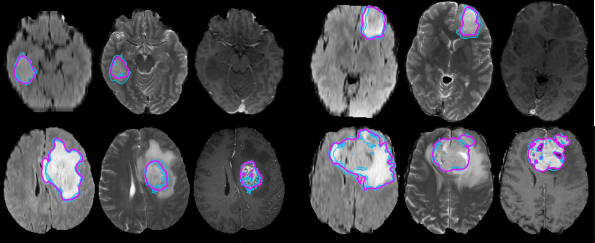
\includegraphics[width=0.99\textwidth]{brats.png}
  \caption{Examples from the BRATS dataset. Annotation of individual experts are in blue, consensus segmentations are in pink. Taken from \cite{menze15}}
  \label{fig:brats}
\end{figure}

\section{Problem definition and thesis statement}

Applying state-of-the-art \gls{dl} methods to segmentation of medical images poses important practical difficulties.
In particular, the task requires a specific medical expertise.
Second, assuming such experts are available and willing to participate to this task, their daily obligations impose a limited time budget.
These two factors largely explain why the field of medical imaging does not benefit from the latest \gls{dl} technologies used in more generic applications \cite{orting19}.
Indeed, the general rule of thumb is: More powerful and flexible model require more training examples.

\textbf{Problem definition}
The present thesis therefore endeavours to address this bottleneck by providing a
fast and intuitive annotation method that allows to generate accurate segmentation of objects of interest on a wide variety of medical imaging modalities.

\textbf{Thesis statement}
Generating pixel-wise annotations of medical sequences over a wide range of modalities is possible.

\section{Organization and Contribution of this Thesis}
The organization of this thesis is summarized below per chapter:

\textbf{Chapter 2} gives a detailed description of the experimental annotation setup.
The datasets that were used in the elaboration and testing of the proposed methods are described.
The requirements of our annotation protocol is then explicitated and justified.
Next, we describe our software solutions, namely a cross-platform and multi-device annotation software, and a web platform with a frontend that allows users to upload annotations, while a backend runs our segmentations algorithms.

\textbf{Chapter 3} gives an overview of the broad litterature related to the present thesis.
In particular, we first give a state-of-the-art of computer vision methods related to segmentation of images and volumes using sparse annotations.
Next, we review several categories of \gls{ml} applicable to the same scenario, namely \gls{ssl}, \gls{pu}, and \gls{da}.
Last, we add some essential theoretical elements that intervene in the proposed solutions.

\textbf{Chapter 4} contains our first segmentation method that relies on the Expected Exponential loss, optimized using a gradient boosting classifier. The probabilities of unlabeled samples are estimated using label propagation.

\textbf{Chapter 5} gives a thorough study of feature extraction methods applicable to the present scenario.
We devise a simple evaluation framework based on a \gls{rf} classifier that operates on superpixels.
As baselines, we implement traditional feature extraction methods, such as \gls{bovw}.
Another baseline considers unsupervised deep feature extraction, where we use a \gls{cnn} trained to classify natural images.
We then implement various methods based on \gls{dl} that integrate motion priors, as well as priors derived from the user-provided point annotations.
Through extensive experiments, we demonstrate the superiority of the \gls{ae} configuration aided by spatial priors over the baselines.
This contribution constitutes a preliminary study that is relevant to the next chapter.

\textbf{Chapter 6} presents an innovative framework based on multi-object tracking.
Concretely, we formulate our segmentation problem as a maximum a-posteriori problem, where the random variable to optimize is the objectness of superpixels.
Using deep features extracted with the best method of the previous chapter, we train an ensemble of decision trees using a sampling method applicable to the \gls{pu} setup.
Next, simple gaussian kernels provide pairwise similarity measures.
These two models allow to define likelihoods of selecting a superpixel given the user's annotations, and transiting from one frame to the next.
Using the network flow paradigm, we then build a graph that connects superpixels according to spatio-temporal relations.
This chapter covers the content of our first journal article \cite{lejeune18}.

\textbf{Chapter 7} continues on the same line as the previous chapter by improving on the foreground prediction model.
Instead of using two components, where the first generates deep features, while the second estimates foreground probabilities, we aim at combining the two in an end-to-end fashion.
We leverage a loss function applicable to the \gls{pu} scenario, where the foreground probabilities are inferred by a deep network configured as a predictor.
As the latter loss function requires accurate class priors to render its full potential, we further devise a strategy to estimate the latter in a self-supervised manner.
In particular, our approach consists in setting an initial upper-bound constant value (possibly misspecified) on the prior, and gradually decrease the latter using as evidence the output of the deep network.
Our algorithm relies on the recursive bayesian estimation paradigm.
This chapter covers the content of our second journal article, currently in preparation.

\textbf{Chapter 8} gives a summary of our contributions, provides general discussions, and concludes by giving an outline on future works.

%%% Local Variables:
%%% mode: latex
%%% TeX-master: "../../main"
%%% End:
